\chapter{Proposed Solutions}

This chapter presents an overview of potential solution approaches relevant to the task of visual outfit evaluation within the field of \acs{CV}. The main goal of the desired solution is to extract features from images, evaluate matching and compute overall compatibility score. 

\section{Overarching Framework}

Based on an in-depth review of related literature, the specific use case and the available resources, a general direction for the solution has been defined: a \acs{GAN}-inspired architecture is most suitable for addressing the challenges of this task.

The generator-like component acts as an outfit creator (template-guided or as a random combiner of clothing items). The discriminator-like component evaluates the quality of these outfits and assigns an aesthetic rating (1-10). The outfit creation process is then iteratively refined based on feedback (e.g. from the scoring model, from the user).

This approach simulates the functionality of a \acs{GAN} without actually implementing a full network and avoiding the complexity of training it. It leverages existing pre-trained models and techniques in a creative way, making it both feasible and resource-efficient. However, without a true generator-discriminator loop, the carefull design of the interaction of generator-like and discriminator-like components is am important task.

\section{Individual Components}

While the overarching framework is clear, the implementation of individual components within this architecture can vary significantly. Therefore, this section explores a range of alternative methods for each key module, analyzing their respective strengths, limitations and applicability.

The different modules in the choosen strategy are illustrated in Figure \ref{fig:workflow-modules} and described bellow.

\begin{figure}[h]
  \centering
  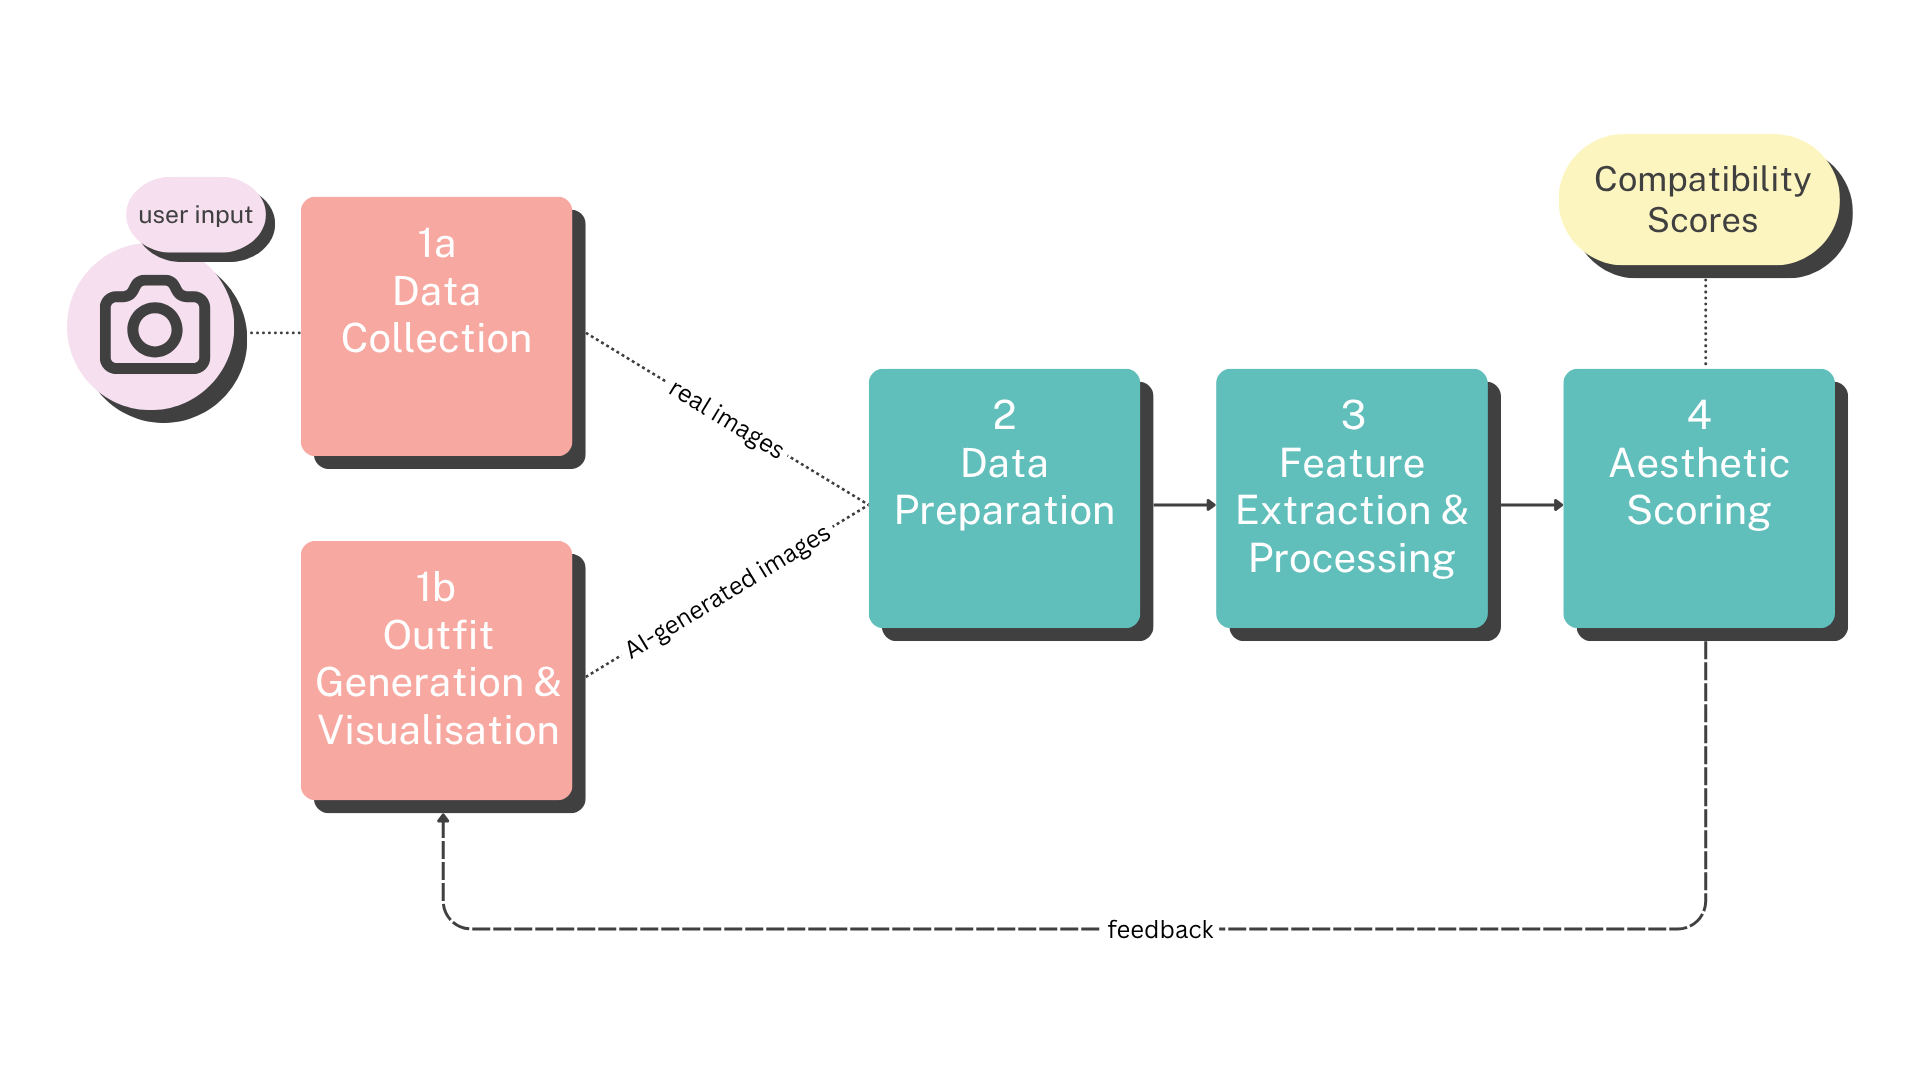
\includegraphics[width=\linewidth]{Abbildungen/workflow-modules.png}
  \caption{\acs{GAN}-Inspired System and its Modules (Workflow)}
  \label{fig:workflow-modules}
\end{figure}

\subsection{Data Collection Module (1a)}

The data collection strategy must align with the chosen method to learn data representations. In this work, two relevant approaches are considered: \acs{NC-SSL} and \acs{SCL}. These methods influence how data should be organized.

\vspace{0.5cm}

\textbf{Positive Pairs (\ac{NC-SSL}).}
This approach that relies exclusively on positive sample pairs and data augmentations. These are well-balanced and stylish outfits, typically sourced from fashion experts or curated user sets.

\vspace{0.5cm}

\textbf{Positive and Negative Pairs (\ac{SCL}).}
This learning strategy uses both positive and negative pairs. While the positive examples remain the same as in the previous approach, negative samples consist of visually unappealing outfits (e.g. those with clashing colors, disproportionate silhouettes, excessive layering).

\vspace{0.5cm}

\textbf{Comparative Analysis:}

\vspace{0.5cm}

Both, positive and negative outfit data samples can be sourced from platforms like Pinterest and Google or from public datasets such as DeepFashion, Polyvore and FashionGen. While there are some positive outfit examples available, identifying truly representative positive and negative samples remains difficult. This is because the quality of an outfit is often subjective. This means, that what looks good to one person might not appeal to another. As a result, both positive and negative samples require human evaluation, ideally with personalization in mind. Randomizing outfit pieces can help generate negative examples, but the results are often unrealistic or too obviously mismatched. Moreover, many bad outfits are only subtly off, making them hard to label without contextual knowledge. Collecting a well-balanced dataset, therefore, demands time and careful curation.

\vspace{0.5cm}

\textbf{Selected Approach incl. Justification:}

\vspace{0.5cm}

Due to the challenges in obtaining reliable contrastive data the decision is made to begin with a non-contrastive training strategy, using only known good outfits. This allows the model to first learn what makes an outfit aesthetically and semantically coherent. Once the training is finished and the model can reliably score outfits using the discriminator-like component, the generator-like component creates outfit combinations and recieves scores. Out of these newly generated outfits, only high- or low-scoring examples are selected for further training. This self-bootstrapping strategy gradually improves the model without relying on manually labeled negative samples.

Current approach is also suitable for a possible future phase, where each user is able to provide a personalized outfit history containing both liked and disliked looks. This allows the model to fine-tune its understanding of style preferences on an individual level, using real user behavior as training input for personalized outfit scoring.

Furthermore, in later stages, additional data can be gathered through user-uploaded outfits, styled looks from partner brands, second-hand shops, or stylists, as well as previously \acs{AI}-generated combinations as discribed in the module 1b.

\subsection{Outfit Generation and Visualisation Module (1b)}

A few approaches to generate and display fashion outfits are being explored:

\vspace{0.5cm}

\textbf{Random Outfit Generation.}
As a baseline, outfits can be randomly sampled by selecting items across predefined categories (e.g. top, bottom, shoes, accessories). While these combinations are unstructured, they allow evaluation of the model's ability to detect outfit quality without prior structure.

\vspace{0.5cm}

\textbf{Rule-Based and Template-Guided Generation.}
This approach imposes structural constraints on outfit creation, provides interpretability and guides the generation of coherent outfits. Fashion heuristics and predefined templates are used. For instance, the \href{https://medium.com/@snc5440/the-8-point-rule-of-fashion-31180d957925}{8-Point Rule of Fashion} offers a quantitative framework where each item contributes a defined number of "style points", promoting visual balance and coherence. These constraints can be applied during generation or as a post-processing filter to refine candidate outfits. Additionally, users can personalize the rule system, enabling flexible alignment with subjective fashion preferences.

\vspace{0.5cm}

\textbf{Outfit Visualisation.}
One way to display an \acs{AI}-generated outfit is by using \acs{IDM-VTON} to place segmented clothing items on a person. This virtual try-on network ensures that generated outfits look realistic and contextually appropriate. However, it may not handle all body shapes or poses perfectly or lead to a computational overhead if used extensively.

\vspace{0.5cm}

\textbf{Comparative Analysis:}

\vspace{0.5cm}

\textcolor{red}{text missing}

\vspace{0.5cm}

\textbf{Selected Approach incl. Justification:}

\vspace{0.5cm}

Rules are used as a starting point but allow the model to deviate based on learned patterns. \textcolor{red}{text missing}

\subsection{Data Preparation Module (2)}

Both modules 1a and 1b feed raw images incl. optional metadata (style, weather, event, gender, tags) into an aesthetic scoring model. The data needs to be processed accordingly in this module.

\vspace{0.5cm}

\textbf{Image Data.}
To prepare images several preprocessing steps are involved. The process begins with object detection or clothing item recognition, which identifies garments using models such as YOLOv8, Detectron2, Grounding DINO or fine-tuned EfficientNet. Following detection, segmentation is applied to isolate clothing items from the background using techniques such as \acs{SAM}, Mask R-CNN or SegFormer. Next valuable step is pose estimation and pose normalization, which helps to understand how items are worn and ensures consistent alignment (e.g. mapping a person to a standard pose). Applying this step would make the comparison between outfits more fair and easier (all images in the same pose = easier to judge fit and compatibility). In order to do pose estimation, tools like OpenPose, MediaPipe or HRNet can be used. Once the relevant clothing regions are identified, cropping and background removal is used to focus solely on the garments. This is done by leveraging segmentation results to crop the items and removing the background using models such as U2Net, RemBG or \acs{SAM}. To ensure consistency in the dataset, images are then resized to a typical resolution (e.g. 224x224 or 512x512) and pixel values are normalized (e.g. to a [0, 1] range). Optionally, data augmentation is utilized to improve generalization.

\vspace{0.5cm}

\textbf{Textual Data.}
When raw image data is accompanied by textual metadata such as descriptions, tags, captions or user comments, it is important to preprocess this information to ensure consistency and usefulness. The first step involves cleaning the text, which includes removing special characters, emojis, irrelevant hashtags and links, as well as normalizing whitespace and converting the text to lowercase. Next, the pipeline includes a text filtering stage to remove uninformative or noisy content. Once the text is cleaned and filtered, it undergoes tokenization, which depends on the model in use.

\vspace{0.5cm}

\textbf{Comparative Analysis:}

\vspace{0.5cm}

\textcolor{red}{text missing}

\vspace{0.5cm}

\textbf{Selected Approach incl. Justification:}

\vspace{0.5cm}

\textcolor{red}{text missing}

\subsection{Feature Extraction and Processing Module (3)}

Ensuring that the system learns meaningful relationships between clothing items and aesthetic ratings requires careful feature engineering. This module captures basic visual attributes such as color and texture. It also learns additional, more complex features, such as color harmony, texture matching, balance, contrast and composition. These features align with human intuition about fashion aesthetics. They add depth to the model's understanding of what makes an outfit "good" and are crucial for evaluating outfit quality.

\vspace{0.5cm}

\textbf{Image Data: Fine Tuning.}
This approach takes a single pre-trained model and fine-tunes it so that it is adapted to new data patterns. The model can then perform the desired tasks on its own. A pre-trained ResNet can be taken and continued to be trained on own data to extract complex features from outfit images (e.g. outfit quality, style labels, embeddings).

\vspace{0.5cm}

\textbf{Textual Data.}
After tokenization, the pipeline proceeds with semantic embedding extraction, transforming the processed text into vector representations. Fashion\acs{CLIP} is preferred for fashion-specific contexts, but alternatives such as \acs{CLIP}, BERT, SBERT, Sentence-T5 or \acs{GloVe} can be used. Optionally, metadata fusion can be applied by converting the attributes into descriptive prompts (e.g. “A red wool sweater with a relaxed fit”) or encoding them as key-value pairs for structured input formats.

\vspace{0.5cm}

\textbf{Ensemble Modeling.}
This is a strategy of using multiple pre-trained networks in order to extract diverse features. It combines outputs from multiple feature extractors, focusing on the strengths of different models, and improves robustness and generalization. However, it may increase computational overhead and requires careful fusion of features from different models.

The output includes cleaned images, segmentation masks and structured metadata.


, which evaluates the generated outfits using learned visual-semantic embeddings (e.g., from FashionCLIP) and learned similarity metrics.



Based on that, the module also refines the features to better represent the outfit's aesthetic qualities. To process the extracted features, an \acs{MLP} can be implemented.

\vspace{0.5cm}

\textbf{Comparative Analysis:}

\vspace{0.5cm}

\textcolor{red}{text missing}

\vspace{0.5cm}

\textbf{Selected Approach incl. Justification:}

\vspace{0.5cm}

\textcolor{red}{text missing}

\subsection{Aesthetic Scoring Module (4)}

This module uses the processed features to predict an aesthetic score. There are two options:

\begin{enumerate}
   \item It can be a simple linear layer or another \acs{MLP} layer to output a score between 0 and 1, which can be scaled to a percentage.
   \item Siamese network can be used to learn similarity-based scoring. This approach allows for meaningful comparisons between outfits, clustering similar outfits and separating dissimilar ones. The quality of the embedding space depends on the diversity of the dataset.
\end{enumerate}

\vspace{0.5cm}

\textbf{Comparative Analysis:}

\vspace{0.5cm}

\textcolor{red}{text missing}

\vspace{0.5cm}

\textbf{Selected Approach incl. Justification:}

\vspace{0.5cm}

\textcolor{red}{text missing}

---------------------------
Both of the explained ideas can be combined. First, multiple specialized models are pre-trained (e.g. a CLIP for semantics, a pose-sensitive model, a garment classifier). Later, an ensemble fusion model is fine-tuned 
on your task (e.g. outfit scoring, quality ranking, similarity).
This way, your Feature Extraction Module is not just plug-and-play — it's a powerful fashion intelligence layer.
Suggestion:
- Start with simpler features like color harmony and balance, which can be computed using computer vision techniques.
- Use pre-trained models or libraries (e.g., ColorThief) to analyze color palettes.
- Gradually incorporate more complex features as the system evolves.
- Start with a small ensemble of two or three models (e.g., one for global features and one for local details).
- Use late fusion (e.g., concatenating outputs) or attention mechanisms to combine features effectively.

Future Research Directions (For Thesis): Investigate the use of machine learning to *dynamically* adjust compatibility rules based on the current outfit's characteristics. Develop a system that allows users to provide more detailed style preferences and integrate these preferences into the generation process. Extend the system to generate outfits that synthesize elements from multiple existing style guidelines, creating unique and novel combinations. - While the output is visually appealing, integration notes suggest a further refinement of the compatibility criteria, potentially incorporating factors like color palettes, silhouette considerations, and formality level.  The system performs well with common garment types - shirts, pants, dresses - but struggles with more complex combinations.

- Use Siamese networks or triplet loss to create an embedding space where similar outfits are closer together.
- Incorporate additional features (e.g., color harmony, balance) into the scoring process.


Key Takeaways
1. Focus on Feasibility: Avoid computationally expensive tasks (e.g., training a GAN) and leverage pre-trained models wherever possible.
2. Prioritize Key Features: Begin with essential features like color harmony, balance, and similarity-based scoring before adding complexity.
3. Iterative Development: Develop the system incrementally, starting with a simple prototype and refining it based on feedback.
4. User-Centric Design: Ensure the final product is engaging and useful for users, with opportunities for personalization and interaction.

proposed a translation-based neural fashion compatibility model which contained three parts: (1) first mapped each item into a latent space via two CNN for visual and textual modality, (2) encoded the category complementary relations into the latent space, and (3) minimized a margin-based ranking criterion to optimize both item embeddings and relation vectors jointly.

Score compatible with me
Score compatible with every other piece I am wearing or could buy

compatibility clothing with me and clothing with eachother

items of clothes (segmented)
whole outfit
person segmented

relations (scores)


splitting it up? possibility
explainable AI -> highlight the least compatible item


The final section provides a justification for the selected combination of techniques, aligning each choice with the project goals and practical constraints.